\documentclass{article}
\usepackage[utf8]{inputenc}

\usepackage{tabularx}
\usepackage{graphicx}
\usepackage{adjustbox}
\usepackage{hyperref}
\usepackage{etoolbox}
\usepackage{changepage}
\usepackage{float}
\usepackage{amsmath}

\usepackage[disable]{todonotes}
%use this line instaed to hide todo's
%\usepackage[disable]{todonotes}

\usepackage{cleveref}

\title{Halbleiterphysik Fragenkatalog}
\author{Constantin Schieber\\Benedikt Tutzer}
\date{August 2020}

%\patchcmd{\subsubsection}{\normalsize}{\normalsize}{\typeout{same line subsec f}}{\typeout{same line subsec failed}}%
%\patchcmd{\subsubsection}{\bfseries}{}{\typeout{same line subsec f}}{\typeout{same line subsec failed}}%

\newtoggle{aftersection}
\preto{\section}{\filbreak\global\toggletrue{aftersection}}
\preto{\subsection}{\iftoggle{aftersection}{\global\togglefalse{aftersection}}{\filbreak}}
\newcommand{\clearpageafterfirst}{%
  \gdef\clearpageafterfirst{\clearpage}%
}


\begin{document}


\maketitle
\vfill
Diese Ausarbeitung ist zur Vorbereitung auf die m\"undliche Pr\"ufung im August 2020 entstanden. Sie kann gern auf overleaf aktuell gehalten werden.\\

\begin{center}\href{Overleaf public link}{https://www.overleaf.com/4852512811wdbqyxrbkgyb}\end{center}

\newpage
\tableofcontents
\newpage

%--------------------------------------------------------------------------------
%--------------------------------------------------------------------------------
%--------------------------------------------------------------------------------
\section*{Overview}
\addcontentsline{toc}{section}{Overview}    %Makes the above section appear in the table of contents


\begin{center}
\begin{table}[H]
%\begin{adjustwidth}{-3cm}{-3cm}
\begin{adjustbox}{width=\textwidth}
\centering
\begin{tabular}{lcccccccc}
Frage                & 02.16 & 01.28 & 02.19 & 03.04 & 03.05 & 03.21 & 01.16 & Katalog\\
                     & 2010  & 2014  & 2019  & 2019  & 2019  & 2019  & 2020 & \\
                     \hline
\ref{k1:photoEf} Photo-Effekt &&&&&&&& X \\
\ref{k1:comptonEf} Compton-Effekt &&&&&&&& X \\
\ref{k1:dispersionsrelation} Dispersionsrelation für Halbleiter && X &&& X & X & X & \\
\ref{k1:schrGl} Schrödinger Gleichung&&&& X &  & X & X & X \\
\ref{k1:ekdiag} e(k) Diagramm &&&&&&&& X \\
\ref{k1:pottopf} Unendlich tiefer Potentialtopf & X &&&&&&& X \\
\ref{k1:tunnEf} Tunneleffekt&&&&&&&X & \\
\ref{k2:metalle} Unterschied Halbleiter vs Metalle &&&&&&&& X\\
\ref{k2:festkorper} Grund für Festkörperbildung & X &&&&&&& X\\
\ref{k2:leitungsBand} Leitungsband, Valenzband, Ef aufzeichnen && X & X &&&&& \\
\ref{k2:kroningpenny} Kroning Penny Modell &&&&&&&& X \\
\ref{k2:entstehungHalbleiter} Enstehung der Halbleiter &&&&&&&& X \\
\ref{k2:phononen} Phononen &&&&&&&& X \\
\ref{k3:diffusion} Berechnung Diffusionsspannung & X &&&&&&& X \\
\ref{k3:alleGleichungen} Alle Gleichungen & X &&&&&&& \\
\ref{k3:dotieren} Dotieren &&&&&&&& X \\
\ref{k3:ladungstraegerkonz} Verlauf der Ladungstr\"agerkonzentration &&&&&&&& X \\
\ref{k3:drude} Drude Modell &&&&&&&& X \\
\ref{k3:halleffekt} Hall-Effekt &&&&&&&& X \\
\ref{k3:hallspannung} Hall-Spannung &&&&&&&& X \\
\ref{k3:diffusionsstrom} Diffusionsstrom &&&&&&&& X \\
\ref{k3:stromgleichungen} Stromgleichungen, J\_n, J\_p &&&&&&&& X \\
\ref{k3:shockleyhaynes} Shockley-Haynes Experiment &&&&&&&& X \\
\ref{k3:kontinuitaet} Kontinuit\"atsgleichungen &&&&&&&& X \\
\ref{k4:laser} Wie funktionieren Laser & X &&&&&&& X\\
\ref{k4:inUndIndirekt} Direkter und Indirekter Halbleiter&&& X &&&&& X \\
\ref{k4:zustandsDichte} Zustandsdichte und Besetzungswahrscheinlichkeit && X &&&&& X \\
\ref{k5:pn} PN-\"Ubergang && X & X & X &X&X&& X \\
\ref{k5:diode} Diodenkennlinie &&&&&&&& X \\
\ref{k5:pnBand} Banddiagramm f\"ur PN ohne Spannung  && X &&&&&& \\
\ref{k5:tunnelDiode} Tunneldiode&&& X && X & X & X & X \\
\ref{k5:tunnelEffekt} Tunneln Allgemein&&&&& X &&& X\\
\ref{k5:schottky} Schottky-Kontakt-Diode &&&&&&&& X \\
\ref{k5:backward} Backward-Diode &&&&&&&& X \\
\ref{k5:heterostrukturen} Heterostrukturen &&&&&&&& X \\
\ref{k6:bipolar} Funktion von Bipolartransistoren & X &&&&&&& X \\
\ref{k6:mosInversion} MOS-Struktur & X && X &&&&& \\
\ref{k6:diffusionsdreieck} Diffusions-Dreieck beim Transistor &&&&&&&& X \\
\ref{k6:fet} Feldeffekt-Transistor &&&&&&&& X \\
\ref{k6:mosfet} MOS-FET &&&&&&&& X \\
\ref{k6:mesfet} MES-FET &&&&&&&& X \\
\ref{k6:early} Early-Effekt &&&&&&&& X \\
\ref{k6:jfet} JFET &&&&&&&& X \\

\hline

\hline

\end{tabular}
\end{adjustbox}
%\end{adjustwidth}
\caption{Mündliche Prüfungsfragen aus diversen Aufzeichnungen der FET.}
\end{table}
\end{center}

%--------------------------------------------------------------------------------
%--------------------------------------------------------------------------------
%--------------------------------------------------------------------------------
\section{Physikalische Grundlagen - Kapitel 1}
\subsection{Photo-Effekt \todo{0x}}\label{k1:photoEf}
Wenn Licht auf reine Metalle trifft und dabei die Frequenz des Lichts eine gewisse Schwelle überschreitet werden Elektronen aus dem Metall gelöst.

\begin{figure}[H]
    \centering
    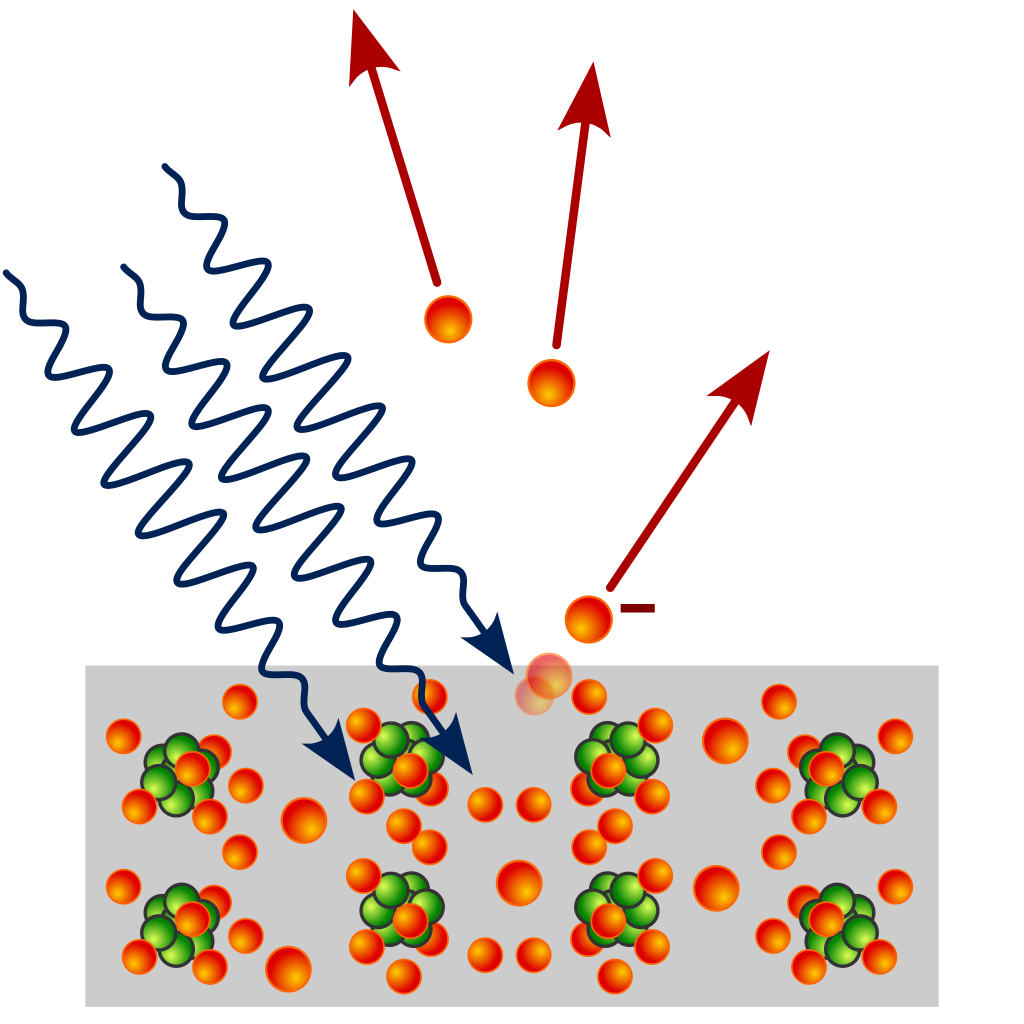
\includegraphics[width=0.33\textwidth]{fig/photoeffect}
    \caption{Photoeffekt}
    \label{fig:photoeffect}
\end{figure}

\subsubsection{Austrittsarbeit}
Die Energie von Licht hängt mit dessen Frequenz zusammen: $\hbar \cdot f$
Die Zahl der emittierten Elektronen ist proportional zur Energie des Lichts.

Das Elektron aus dem Metall muss zum Austreten die \textit{Austrittsarbeit}: $W = h \cdot f_g$ verrichten können.
Hat ein Photon also nicht mindestens die Frequenz $f_g$, oder besser noch $f > f_g$, dann kann auch kein Elektron freigesetzt werden.

Die Austrittsarbeit kann auch experimentell (Lenard, 1992) beobachtet werden: $e|U| = h| f - f_g|$
\begin{figure}[H]
    \centering
    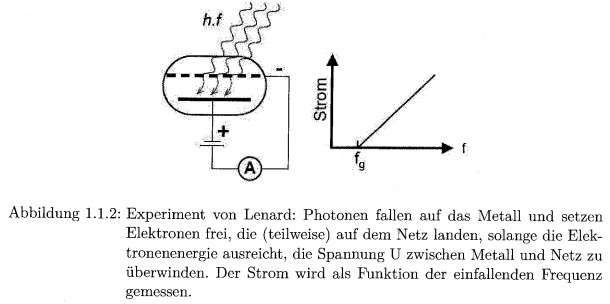
\includegraphics[width=0.5\textwidth]{fig/photoExperiment}
    \caption{Photoeffekt}
    \label{fig:photoeffectExperiment}
\end{figure}

\subsection{Compton-Effekt \todo{0x}}\label{k1:comptonEf}
UV-Licht trifft auf Metall. Im Streulicht (der Reflexion), ist dann nicht nur die Primärfrequenz sondern auch noch längerwellige Frequenz nachweisbar.   
Compton Effekt (eben das Auftreten dieser längerwellige Frequenz) ist nicht allein durch das Wellenbild des Photons erklärbar.
Über das Teilchenbild ist das Phänomen allerdings vollständig erklärbar indem man den elastischen Stoß zwischen Photon und Elektron betrachtet.

\begin{figure}[H]
    \centering
    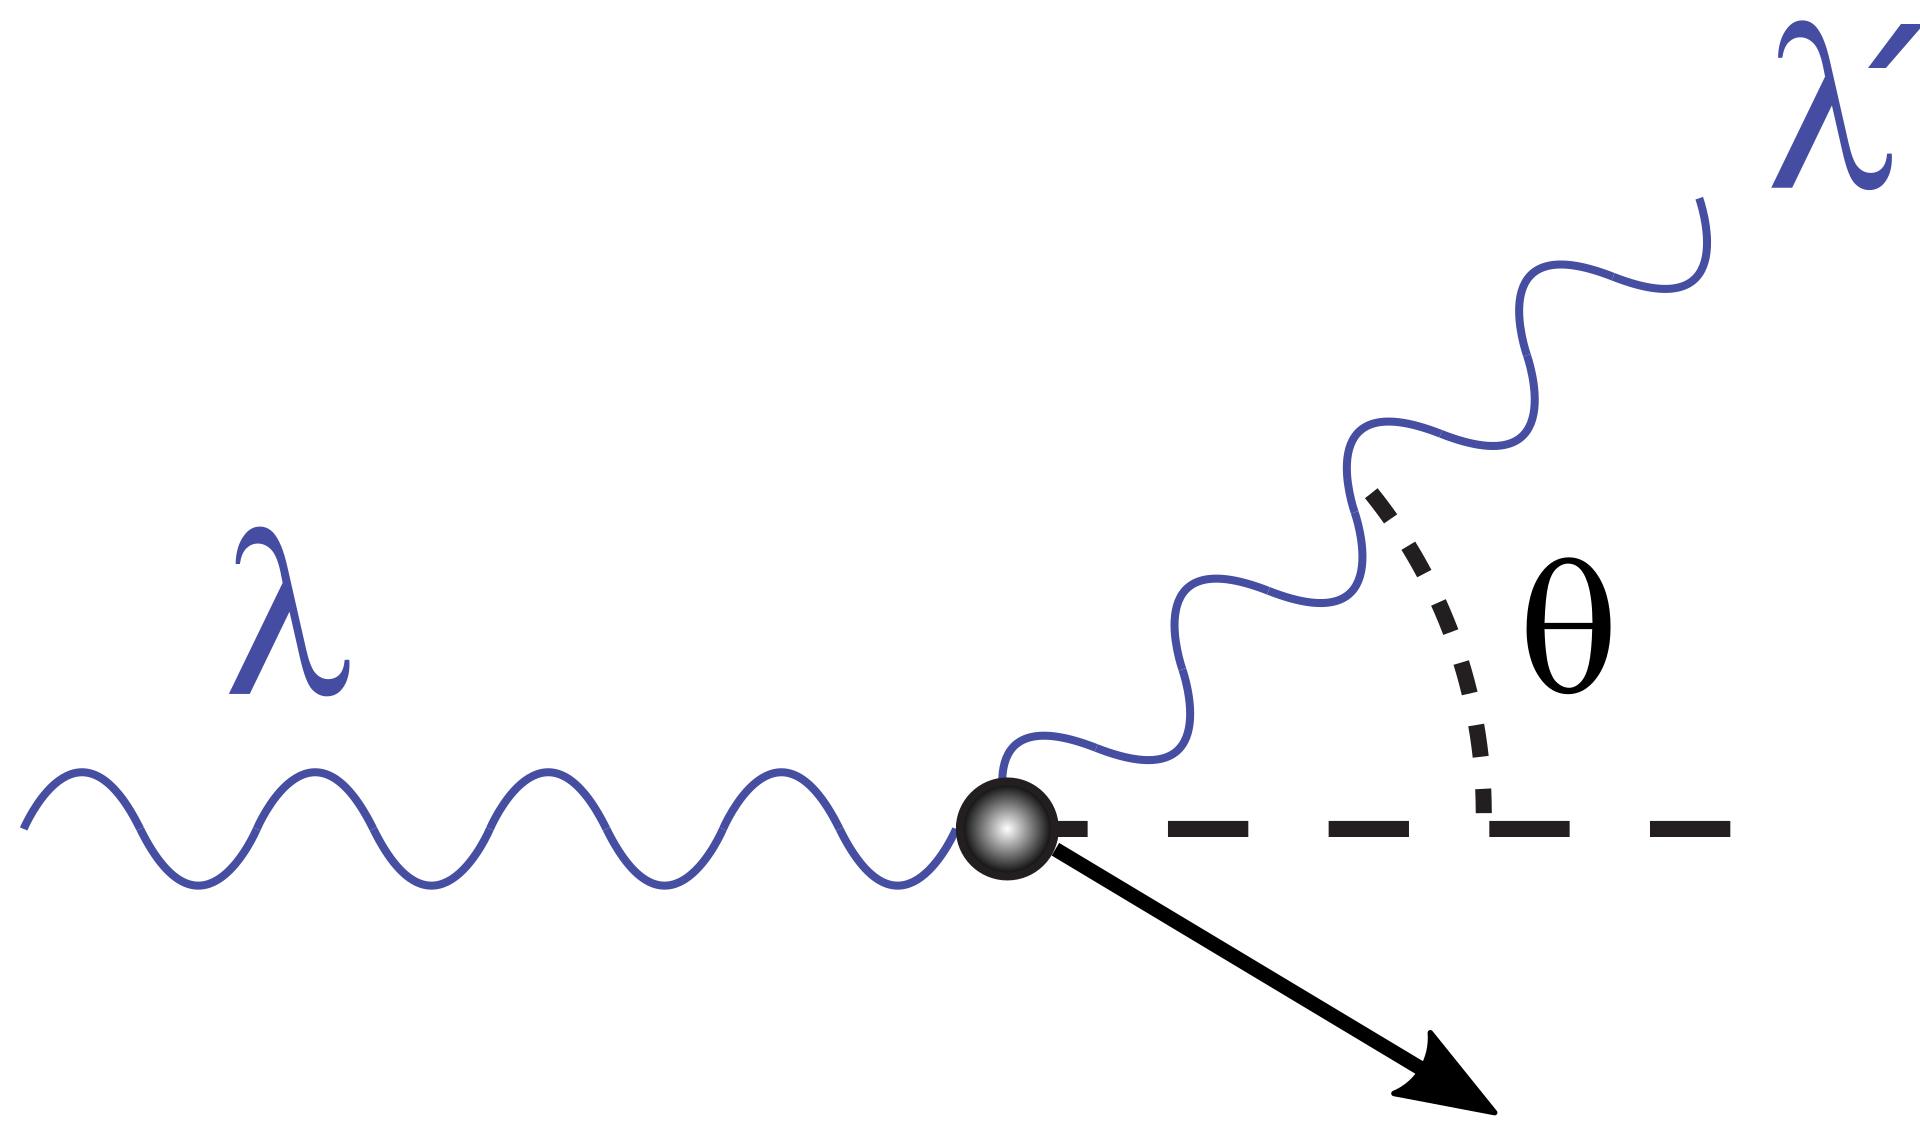
\includegraphics[width=0.5\textwidth]{fig/compton}
    \caption{Compton-Effekt}
    \label{fig:comptonEffect}
\end{figure}

\subsubsection{Durch welche zwei Gleichungen lässt sich der Compton-Effekt erklären?}
Durch den Energie und Impulserhaltungssatz. 

\begin{enumerate}
    \item $E_e$ ... kinetische Energie
    \item $\vec{p}_e$ ... Impuls des Compton-Elektrons (welches heraus geschlagen wird)
    \item $\vec{k}$ ... Wellenvektor zeigt die Ausbreitungsrichtung des Photons
\end{enumerate}
\begin{equation}
    \hbar \omega_0 = \hbar \omega_{sc} + E_e
\end{equation}

\begin{equation}
    \hbar \vec{k}_0 = \hbar \vec{k}_{sc} + \vec{p}_e
\end{equation}

\subsubsection{Was beweist der Compton-Effekt?}
Der Compton-Effekt ist ein direkter Beweis, dass Photonen nicht nur die Energie $\hbar \omega$, sondern auch den Impuls $\hbar k$ haben.

\subsection{Dispersionsrelation \todo{4x}}\label{k1:dispersionsrelation}
\subsubsection{Bandstruktur}
\subsubsection{Bandlücke}
\subsubsection{direkt/ indirket}
\subsubsection{Effektive Masse (was ist schwerer, Elektron im Leitungsband oder Loch im Valenzband?)}
\subsubsection{Wo liegt k=0, E=0 für dirket/indirekt}
\subsubsection{wo ist Elektron nach anheben ins Leitungsband bei indirektem HL (energetisch günstig!)}
\subsubsection{Gedankenexperiment: wenn Elektron in Leitungsband, und Valenzband voll besetzt, was passiert, wenn man HL abkühlt?}

\subsubsection{Zusammenhang zwischen Energie E und der Kreiswellenzahl k}
\subsubsection{Lösung für freies Teilchen}
\subsubsection{Dispersion im Halbleiter}

\subsubsection{Skizze Valenzband, Leitungsband, Ferminiveau}
\subsubsection{Direkter indirekter Halbleiter}
\subsubsection{E(k) Diagramm einzeichen k = 0 , E = 0}

\subsubsection{Elektronen und Löcher}
Was bewegt sich wie, Loch zu Elektron, Elektron zu Loch

\subsubsection{Effektive Masse, Definitionen, Masssen}


\subsection{Schrödinger Gleichung \todo{3x}}\label{k1:schrGl}
\subsubsection{Herleitung für freies Teilchen}
Basiert auf der Annahme dass Welle - Teilchen - Dualismus exisiert. 

Dann gilt nämlich sowohl $E = \hbar \omega$ als auch $p = \hbar * k$

\subsubsection{Spezialfall der Schrödingergleichung für ein \textit{freies} Teilchen:}
\begin{equation}
    -\frac{\hbar^2}{2m} \times \frac{\partial^2}{\partial x^2} \Psi(x,t)  = i \hbar \times \frac{\partial}{\partial t} \Psi(x,t)
\end{equation}

\subsubsection{Allgemeine Form der Schrödingergleichung für ein Teilchen:}

\paragraph{Für den eindimensionalen Fall:}
\begin{equation}
    -\frac{\hbar^2}{2m} \times \frac{\partial^2}{\partial x^2} \Psi(x,t) + V(x,t) \times \Psi(x,t) = i \hbar \times \frac{\partial}{\partial t} \Psi(x,t)
\end{equation}

\paragraph{Für den dreidimensionalen Fall:}

Einfach alles durch Vektoren austauschen mit: 

\begin{equation}
    \frac{\partial^2}{\partial x^2} \longrightarrow \frac{\partial^2}{\partial x^2} + \frac{\partial^2}{\partial y^2} + \frac{\partial^2}{\partial z^2} \equiv \Delta
\end{equation}
und 
\begin{equation}
    E = \frac{\vec{p}^2}{2m} + V(\vec{x})
\end{equation}
was dann schließlich einfach

\begin{equation}
    -\frac{\hbar^2}{2m} \times \Delta \Psi(\vec{x},t) + V(\vec{x},t) \times \Psi(\vec{x},t) = i \hbar \times \frac{\partial}{\partial t} \Psi(\vec{x},t)
\end{equation}
ergibt. Man sieht, es ändert sich eigentlich nicht viel - einfach aus dem Ort \textit{x} und dem Impuls \textit{p} einen Vektor machen und logisch durchgehen wo diese ersetzt werden müssen. 

\begin{enumerate}
    \item Warum kann das Potential nicht von der Zeit abhängen
\end{enumerate}

\subsubsection{Dispersionsrelation für ein freies Teilchen}

\subsubsection{Aufstellen der Zeitabhängingen und Zeitunabhängigen Lösung}

\subsubsection{Einzelne Terme erklären}
\begin{enumerate}
    \item Was ist Phi
    \item Welche Abhängigkeiten (x, t) warum
    \item Was ist das Potenzial?
    \item Von was ist das Potenzial abhängig (x, t)
    \item Freies Teilchen in der Schrödingergleichung für V = 0
    \item Lösung der Schrödingergleichung für ein freies Teilchen im E(K) Diagramm
\end{enumerate}

\subsection{e(k) Diagramm \todo{0x}}\label{k1:ekdiag}

\subsection{Unendlich tiefer Potentialtopf \todo{1x}}\label{k1:pottopf}

\subsection{Tunnel-Effekt \todo{1x}}\label{k1:tunnEf}
\begin{enumerate}
    \item Barriere mit Potenzialschwelle in der Höhe von $V$ und mit der Breite $d$
    \item Teilchen mit Energie kleiner als $V$
    \item Klassische Mechanik: Teilchen wird \textit{immer} reflektiert
    \item Quantenmechanik: Teilchen durchdringt die Barriere mit einer gewissen Wahrscheinlichkeit (oder wird andernfalls relfektiert) $\rightarrow$ \textit{Es tunnelt}
\end{enumerate}
\begin{figure}
    \centering
    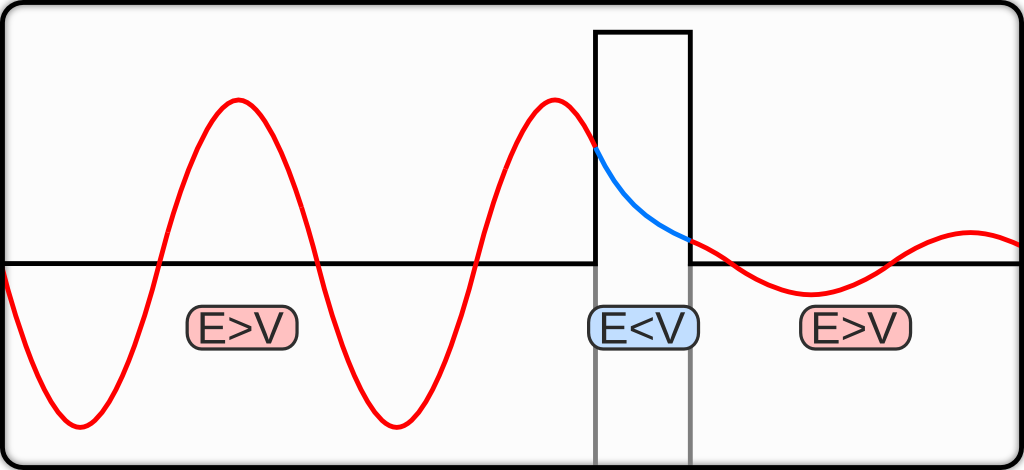
\includegraphics[width=0.66\textwidth]{fig/tunneleffektwiki.png}
    \caption{Schematische Darstellung des Tunneleffekts:
Ein Teilchen trifft von links kommend auf eine Potentialbarriere. Die Energie des getunnelten Teilchens bleibt gleich, nur die Amplitude der Wellenfunktion wird kleiner und somit die Wahrscheinlichkeit, das Teilchen aufzufinden.}
    \label{fig:tunneleffekt}
\end{figure}

Der Tunneleffekt wird für Dinge wie SRAM (Floating Gate MOS-FETs) und Rastertunnelmikroskope ausgenutzt. 

\subsubsection{Herleitung der Tunnelwahrscheinlichkeit}
Ist scheinbar noch nie gekommen, prinzipiell wird er über die zeitunabhängige (also stationäre) Schrödingergleichung angesetzt. 
Danach wird entlang der x-Achse zwischen drei Teilen unterschieden:
\begin{enumerate}
    \item I: Vor der Barriere, $V = 0$
    \begin{enumerate}
        \item Für die Wellenfunktion: $\varphi_I(x) = A_1e^{ikx} + A_2e^{-ikx}$ (Superposition von einer planaren nach rechts bzw. links laufenden Welle - die linke steht für den reflektierten Anteil)
    \end{enumerate}
    \item II: In der Barriere, $E > V \rightarrow E - V$ (Energie der Welle ist größer als die Barriere)
    \begin{enumerate}
        \item In der Barriere gibt es nicht wirklich eine Wellenfunktion, sondern einfach einen exponentiellen Verlauf, weswegen dort die komplexe Zahl im exponenten fehlt:
        \item $\varphi_{II}(x) = B_1e^{\kappa x} + B_2e^{-\kappa x}$
    \end{enumerate}
    \item III: Nach der Barriere $V = 0$ geht es weiter wie gewohnt
    \begin{enumerate}
        \item Nur neue Amplituden müssen wir einführen, da ja die Wahrscheinlichkeit eines Antreffens niedriger sein wird:
        \item $\varphi_{III}(x) = C_1e^{ikx} + C_2e^{-ikx}$
    \end{enumerate}
\end{enumerate}

Jetzt kann man einige Überlegungen für die Amplituden anstellen:
\begin{enumerate}
    \item $A_1$ und $A_2$ sind uns beide nicht bekannt, aber wir können mal normieren $A_1 = 1$
    \item $B_1$ und $B_2$ sind uns beide nicht bekannt
    \item $C_1$ ist die Welle die nach rechts läuft - die behalten wir! $C_2$ wäre der reflektierte Anteil, aber nach dem Tunneln gibt es keine Reflexion mehr, also gilt $C_2 = 0$
\end{enumerate}

%--------------------------------------------------------------------------------
%--------------------------------------------------------------------------------
%--------------------------------------------------------------------------------
\section{Periodische Festkörperstrukturen - Kapitel 2}
\subsection{Unterschied Halbleiter vs Metalle \todo{0x}}\label{k2:metalle}
Metalle: Gute Leitf\"ahigkeit aufgrund des vorhandenen Elektronengas. Bereits mit wenig Energie werden genug Elektronen gel\"ost um zu leiten.\\
Halbleiter: Leitf\"ahigkeit liegt zwischen Leitern und Nichtleitern. (Bandl\"ucke $< 1eV$)\\
Nichtleiter (Bandl\"ucke $> 3eV$).\\
Siehe \Cref{fig:bandLHL}.
\begin{figure}[h]
        \centering
        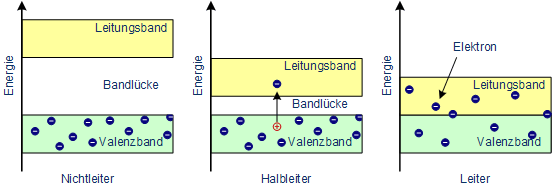
\includegraphics[width=0.6\textwidth]{fig/baendermodellLHL}
        \caption{B\"andermodell f\"ur Nichtleiter, Halbleiter und Leiter}
        \label{fig:bandLHL}
\end{figure}

\subsection{Grund für die Bildung von Festkörpern \todo{1x}}\label{k2:festkorper}
Ausgang: Wasserstoffatom als Modellsubstanz. Hier gillt eine sph\"arische Wellenfunktion:
\begin{equation}
    \Psi_H(r) = C \cdot e^{(-\frac{r}{a_0})}
\end{equation}
mit $a_0$ Bohr'scher Radius.\\
Daraus wird ein 2D-Gitter aus Automen gebaut, wobei davon ausgegangen wird dass Bindungen nur zwischen n\"achsten Nachbaren auftritt (tight binding Methode).
Die Energieskala wird so gew\"ahlt, dass der Zustand des neutralen Atoms (das Elektron befindet sich direkt am Atom) dem Energienullpunkt entspricht.\\
Gibt man einen weiteren Wasserstoffkern dazu, kann sich das Elektron entweder so positionieren, dass es beide Potentiale sp\"urt (seine Energie wird abgesenkt, $\Psi_1$, bindender Zustand) oder so, dass es sich nur bei den Ionen aufhält (seine Energie wird angehoben, $\Psi_2$, anti-bindender-Zustand).
\begin{center}
    \begin{align*}
        \Psi_1 &= \Psi_H(r_1)+\Psi_H(r_2)\\
        \Psi_2 &= \Psi_H(r_1)-\Psi_H(r_2)
    \end{align*}
\end{center}
\begin{figure}[h]
        \centering
        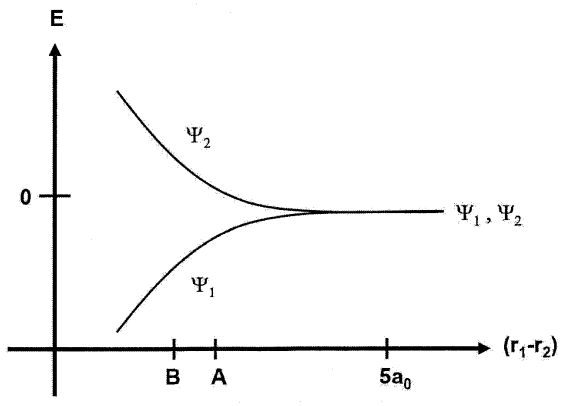
\includegraphics[width=0.6\textwidth]{fig/atomdistanz}
        \caption{Energie des bindenden- und anti-bindenden Zustands in Abh\"angigkeit vom Abstand der Atome. A = metall, B = halbleiter}
        \label{fig:atomdistanz}
\end{figure}
\subsection{Leitungsband, Valenzband, Ef aufzeichnen \todo{2x}}\label{k2:leitungsBand}

Siehe \Cref{fig:bandLHL}. Ef?

\subsection{Kroning Penny Modell \todo{0x}}\label{k2:kroningpenny}
Erkl\"aren, Skizzen, Rechenvorgang, grafische L\"osung, Herleitung e(k) Diagramm

\subsection{Entstehung der Halbleiter \todo{0x}}\label{k2:entstehungHalbleiter}

Verschiebt man die inneren Atome einer periodischen atomaren Anordnung so, dass der Abstand eines Paares kleiner wird als der Abstand der anderen Atome, \"andert sich die Verteilung der Energieniveaus. Die Bindungsenergie des n\"aheren Paares steigt, der Abstand zwischen bindendem und anti-bindendem Zustand wird wesentlich gr\"o{\ss}er. F\"ugt man weitere Atome hinzu, belibt der gr\"o{
\ss}ere Energieabstand erhalten. Die weiteren Energieniveaus gruppieren sich um die bindende und anti-bindende Energie (\Cref{fig:energieHalbleiter}).

\begin{figure}[h]
        \centering
        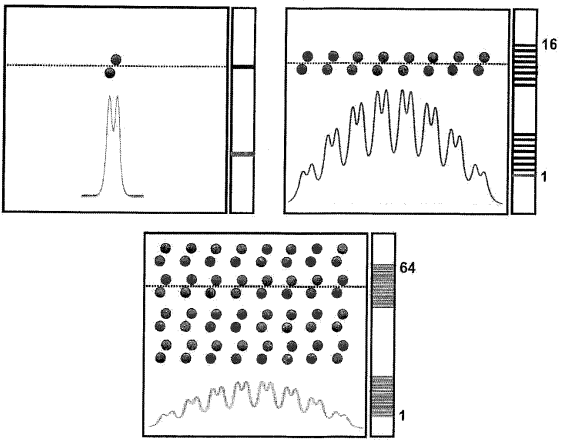
\includegraphics[width=0.6\textwidth]{fig/energieHalbleiter}
        \caption{Energiegruppierung in Halbleitern}
        \label{fig:energieHalbleiter}
\end{figure}

Es entstehen immer dann Halbleiter, wenn sowohl k\"urzere als auch l\"angere Bindungsl\"angen existieren. Erreichen kann man das z.B. durch inneinanderstellen von zwei Gittern (\Cref{fig:gitterstrukturen}).

\begin{figure}[h]
        \centering
        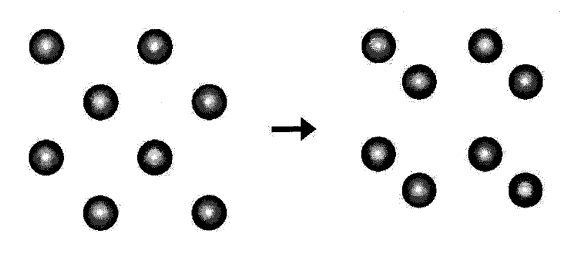
\includegraphics[width=0.6\textwidth]{fig/gitterstrukturen}
        \caption{Anordnung des zweidimensionalen Gitters}
        \label{fig:gitterstrukturen}
\end{figure}

Auf Grund der st\"arkeren Bindungen sind Halbleiter h\"arter als Metalle. Bei $T=0K$ haben sie keine Leitf\"ahigkeit.
Das untere Band (Name Valenzband) ist vollständig mit Elektronen besetzt, das obere Band (Leitungsband) ist leer.
Es gibt gleich viele Zustände im unteren und oberen Band. Wenn Ladungsträger ins obere Band angeregt werden, können
sie sich frei bewegen und führen zu einer hohen Leitfähigkeit.
\subsection{Phononen \todo{0x}}\label{k2:phononen}

%--------------------------------------------------------------------------------
%--------------------------------------------------------------------------------
%--------------------------------------------------------------------------------
\section{Transporteffekte in Halbleitern - Kapitel 3}

\subsection{Berechnung der Diffusionsspannung \todo{1x}}\label{k3:diffusion}
Feldst\"arke (Poissongleichung) integrieren und die Skizzen von pn-\"Ubergang, elektrischer
Feldst\"arke und Spannungsverlauf.

\subsection{Alle Gleichungen (2x Stromgleichung, 2x Kontinuitätsgleichung, 1x Poisson-Gleichung) \todo{1x}}\label{k3:alleGleichungen}

\subsection{Dotieren \todo{0x}}\label{k3:dotieren}

\subsection{Verlauf der Ladungstr\"agerkonzentration als Funktion der Temperatur \todo{0x}}\label{k3:ladungstraegerkonz}

\subsection{Drude Modell \todo{0x}}\label{k3:drude}

\subsection{Hall-Effekt \todo{0x}}\label{k3:halleffekt}
Metallplatte aufzeichnen mit Koordinatensystem und I, B, und F bzw. E als Vektoren.
Kurz beschreiben was im p-HL und n-HL passiert.
Erk\"aren warum der Strom nur in eine Richtung flie{\ss}en kann.

\subsection{Hall-Spannung \todo{0x}}\label{k3:hallspannung}

\subsection{Diffusionsstrom \todo{0x}}\label{k3:diffusionsstrom}

\subsection{Stromgleichungen \todo{0x}}\label{k3:stromgleichungen}

\subsection{Shockley-Haynes Experiment \todo{0x}}\label{k3:shockleyhaynes}
    \subsubsection{Schlatung aufzeichnen} Oszi und Spannungsquelle nicht vergessen
    \subsubsection{Kurve aufzeichnen und erkl\"aren was abgelesen werden kann}

\subsection{Kontinuit\"atsgleichungen \todo{0x}}\label{k3:kontinuitaet}

	\subsection{Intrinsische Ladungsträgerdichte $n_i$ + Gleichung $n \cdot p=n_i^2$ }
	Die intrinsische Ladungsträgerdichte beschreibt die Eigenleitungsdichte eines Halbleiters. Sie bestimmt den Mindestwert der elektrischen Leitfähigkeit.  
	Bei Halbleitern die auf den absoluten Nullpunkt gekühlt werden, sind alle Elektronen im Kristllgitter gebunden. Erst wenn die Temperatur erhöht wird, können Elektronen durch die nun zur Verfügung stehende thermische Energie vom Valenz- ins Leitungsband gehoben werden.
	Durch Rekombination wandern die Elektronen vom Leitungsband wieder ins Valenzband, dabei wird Energie freigesetzt. 
	Im thermodynamischen Gleichgewicht finden nun Rekombination und Generation von Elektronen statt. Diese sollten im Mittel gleich oft verkommen - um eben ein Gleichgewicht zu erhalten.
	Das bedeutet auch, dass die \textit{Anzahldichte} von freien Elektronen im Mittel konstant ist. 
	Die Eigenleitungsdichte $n_i$ setzt sich also aus der durchschnittlichen Anzahl an freien Elektronen $n$ und Löchern $p$ zusammen. Aufgrund des \textit{Massenwirkungsgesetzes}\footnote{Bei einer reversiblen Reaktion im chemischen Gleichgewicht hat der Quotient aus Ausgangsstoff (Elektron) und Reaktionsprodukt (Loch) einen festen charakteristischen Wert, auch Gleichgewichtskonstante genannt.} kann man schreiben:
	\begin{equation}
	    n_i^2 = n \cdot p
	\end{equation}
	Allerdings ist zu bedenken, dass sich die Eigenleitungsdichte massiv mit der Temperatur verändert, da durch die thermische Energie auch mehr Elektronen im Leitungsband zur Verfügung stehen - das ist auch der Grund warum dotierte Halbleiter ihre typischen Eigenschaften verlieren.
	Zum Beispielt verdoppelt sich $n_i$ bei einem Anstieg von 300 Kelvin auf 310 Kelvin.
	
	Diesen Effekt kann man über folgende Formel beschreiben:
	\begin{equation}
	    n_i^2 = n \cdot p = N_C \cdot N_V e^{-\frac{E_C-E_V}{kT}}
	\end{equation}\label{equ:eigenleitung}
	
	\begin{enumerate}
	    \item $N_C$ ... Bandgewicht des \emph{Leitungsbandes}, also die Zahl der Zustände in $\Delta E$ der Breite kT
	    \begin{enumerate}
	        \item Das Bandgewicht steigt mit der effektiven Masse und mit der Temperatur.
	        \item Höhere Temperatur bedeutet, dass mehr Zustände besetzt sind
	        \item Basiert auf der \textbf{Elektronendichte} $n$
	        \item Wikipedia nennt das die \textbf{Effektive Zustandsdichte} des Leitungsbands
	    \end{enumerate}
	    \item $N_V$ ... Bandgewicht des \emph{Valenzbandes}
	    \begin{enumerate}
	        \item Basiert auf der \textbf{Löcherdichte} $p$
	        \item Wikipedia nennt das die \textbf{Effektive Zustandsdichte} des Valenzbandes
	    \end{enumerate}
	    \item $E_C$ ... Energie der Unterkante des Leitungsbandes
	    \item $E_V$ ... Energie der Oberkante des Valenzbandes
	    \item $k$ ... Boltzmannkonstante
	\end{enumerate}
	
	\begin{enumerate}
	    \item Typische Größen für $n_i$ bei Raumtemperatur (26 Grad, 300 Kelvin)
	    \begin{enumerate}
	        \item Silizium: $1.5 \cdot 10^{10} cm^{-3}$
	        \item Germanium: $2.2 \cdot 10^{13} cm^{-3}$
	    \end{enumerate}
	\end{enumerate}
	
	\subsection{$n_i$ ist Funktion von was? (T und Gap)}
    Wie man in \autoref{equ:eigenleitung} sieht, ist die Eigenleitungsdichte $n_i$ von der Temperatur T abhängig.
    Die Temperaturabhängigkeit verringert sich wenn die Bandlücke, die sich aus $E_G = E_C - E_V$ ergibt, vergrößert. 
    
    Das macht Sinn, denn ein größerer Zähler aus \autoref{equ:eigenleitung} $e^{-\frac{E_G}{kT}}$ kaschiert Änderungen in der Temperatur besser.
    
    \subsubsection{Eigenleitung und Fermi-Niveau}
    Es soll noch erwähnt werden, dass die Eigenleitung $n_i^2$ auch zur Berechnung des Fermi-Niveaus herangezogen werden kann.
    Durch Lösen nach $n_i^2$ von \autoref{equ:eigenleitung} auf und einsetzen in andere Gleichungen kann man das Fermi-Niveau $E_F$ bestimmen bzw. auch zur Berechnung von \textit{p} und \textit{n} heranziehen. 
    Grundaussage ist aber, dass $E_F$ bei Eigenleitung in der Mitte des verbotenen Bandes liegt.
    
%--------------------------------------------------------------------------------
%--------------------------------------------------------------------------------
%--------------------------------------------------------------------------------
\section{Optische Eigenschaften von Halbleitern - Kapitel 4}

\subsection{Laser \todo{1x}}\label{k4:laser}
    \subsubsection{Wie funktionieren HL-Laser?}
    Licht kann von Halbleitern absorbiert und emittiert werden.
    Es gilt die Energieerhaltung: $\hbar \omega = \Delta E$, mit der Kreisfrequenz des absorbierten bzw. emittierten Lichts $\omega$,
    und der Energiedifferenz zwischen Anfangs- und Endzustand des Elektrons $\Delta E$.\\
    Es gibt
    \begin{enumerate}
        \item \emph{Interband\"uberg\"ange}, also \"Uberg\"ange zwischen zwei verschiedenen B\"andern
        \item \emph{Intraband\"uberg\"ange} innerhalb eines Bandes zwischen zwei verschiedenen Energieniveaus
    \end{enumerate}
    Die Wechselwirkung zwischen Elektronen und Photonen kann auf drei Arten geschehen:
    \begin{enumerate}
        \item \emph{Absorption}: Ein Photon mit der richtigen Energie kann in einem quanten-mechanischen System (mit einer gewissen Wahrscheinlichkeit) ein Elektron von einem niederenergetischen Zustand in einen höherenergetischen Zustand heben. Das Photon wird
        dabei vernichtet.
        \item \emph{Spontane Emission}: Ein Elektron in einem angeregten Zustand eines quanten-mechanischen Systems kann spontan ein Photon emittieren. Das Elektron fällt dabei vom höherenergetischen in den niederenergetischen Zustand. So funktionieren LEDs.
        \item \emph{Stimulierte Emission}: Trifft ein Photon auf ein angeregtes System, so kann (mit einer gewissen Wahrscheinlichkeit) ein zweites (identes) Photon erzeugt werden. Das Elektron fällt dabei vom höherenergetischen in den niederenergetischen Zustand.
        So funktionieren LASER (\textbf{L}ight \textbf{a}mplification by \textbf{s}timulated \textbf{e}mission of \textbf{r}adiaton).
    \end{enumerate}
    Beispielhafter Aufbau eines HL-Lasers in \Cref{fig:hlLaser}.
    \begin{figure}[H]
        \centering
        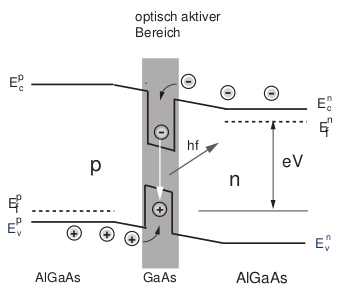
\includegraphics[width=0.6\textwidth]{fig/hlLaser}
        \caption{Aufbau eines HL-Lasers}
        \label{fig:hlLaser}
    \end{figure}
    Die Laserstrahlung liegt energetisch unter der Bandlücke des umgebenden Materials. Die Strahlung kann also problemlos aus dem Halbleiter heraus und wird nicht wieder absorbiert.
    \subsubsection{E(k) Diagramm}
        \begin{figure}[H]
            \centering
            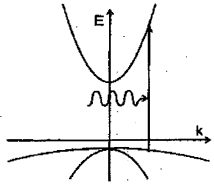
\includegraphics[width=0.3\textwidth]{fig/ekLaser}
            \caption{E(k)-Diagramm f\"ur Laser}
            \label{fig:ekLaser}
        \end{figure}
    \subsubsection{stimulierte Emission}
    Im thermodynamischen Gleichgewicht tritt stets Absorption auf ($Uv(E_1)-f_c(E_2) > 0$), nicht aber wenn der Halbleiter angeregt wird ($Uv(E_1)-f_c(E_2) < 0$), man spricht von Inversion.
    \subsubsection{Verst\"arkerbedingung}
    $E_{F_C}$ Fermi-Niveau Leitungsband\\
    $E_{F_V}$ Fermi-Niveau Valenzband\\
    Bedingung: $E_{F_C} - E_{F_V} > E_G$. ???\\
    Bei $T=0K$ genügt eine beliebig kleine Ladungsträgerinjektion, um die Quasi-Fermi-Niveaus $E_{F_c}$ und $E_{F_v}$ in die Bänder hinein zu verschieben (\Cref{fig:invLaser}) und die Verstärkerbedingung zu erfüllen. Bei Raumtemperatur ist allerdings eine relativ hohe Mindestladungsträgerdichte erforderlich, um Inversion zu erreichen ($ > 10^{18}/cm^3$).
        \begin{figure}[H]
            \centering
            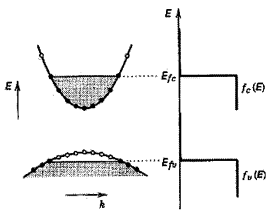
\includegraphics[width=0.3\textwidth]{fig/inversionLaser}
            \caption{Inversion bei $T=0K$}
            \label{fig:invLaser}
        \end{figure}

\subsection{Vergleiche direkte und indirekte Halbleiter \todo{1x}}\label{k4:inUndIndirekt}
    Bei direkten Halbleitern liegt das Maximum des Valenzbandes energetisch genau unter dem Minimum des Leitungsbandes, dies ist z.B. bei
    Galliumarsenid der Fall. Bei indirekten Halbleitern liegen diese ausgezeichneten Punkte bei unterschiedlichen k-Werten (Silizium, Germanium).
    \subsubsection{Wo ist k=0, was bedeutet das?}
    Beim direkten Halbleiter ist $k=0$ dort, wo das minimum des Leitungsbandes und das maximum des Valenzbandes liegen. Sonst???
    \subsubsection{w(k) für freies Teilchen}
    ???
    \subsubsection{Bewegt sich ein e- im Ev bei T=0?}
    ?\\
    Nein, bei $0K$ ist das Valenzband voll besetzt. Elektronen k\"onnen sich nirgends hin bewegen.
    \subsubsection{Wo ist die Masse am größten (Ev, Ec)?}
    ???
    \subsubsection{Gleichung für m*}
    Aufgrund der Auswirkung der Bandstruktur auf die Elektronen im Kristall scheinen diese dort eine andere Masse zu haben, sie wird
    effektive Masse $m^{*}$ genannt.
    \begin{equation}
        \frac{1}{m^{*}} = \frac{1}{\hbar^2}*\frac{d^2E}{dk^2}
    \end{equation}
    \begin{figure}
        \centering
        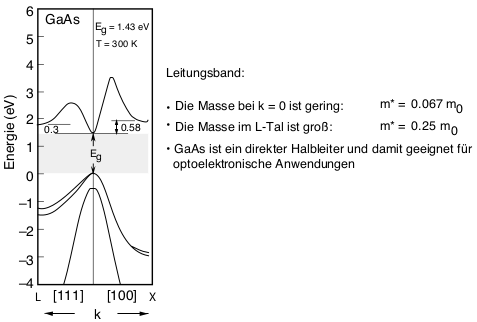
\includegraphics[width=0.8\textwidth]{fig/bandstrukturGaAs}
        \caption{Bandstruktur GaAs}
        \label{fig:bandGaAs}
    \end{figure}
    Betrachtet man die Bandstruktur von z.B. GaAs (\Cref{fig:bandGaAs}), erkennt man dass bei den Wendepunkten die Masse ins unendliche
    gehen w\"urde. Dies passiert aber nicht, in diesen Gebieten braucht es ein anderes Modell, die kp-Theorie.
    Am oberen Rand wird die effektive Masse negativ. Man spricht von einem Loch, die Ladung wird positiv.

\subsection{Zustandsdichte und Besetzungswahrscheinlichkeit \todo{2x}}\label{k4:zustandsDichte}
    Quantensysteme haben diskrete Zust\"ande.
    Die Zustandsdichte $g(E) = \frac{N}{L^3}$ gibt an wie viele Zust\"ande pro eV es zu einem gewissen Energieniveau gibt (Mit $N$ anzahl diskreter Zust\"ande, $L^3$ Volumen des HL).
    Die Besetzungswahrscheinlichkeit, auch Fermi-Verteilung, $P(E)$ gibt die Wahrscheinlichkeit an dass ein Zustand eingenommen wurde.
    Daraus l\"asst sich berechnen, wie viele Leitungstr\"ager vorhanden sind: $n = \int{g(E)*P(E) dE}$
    
    \subsubsection{Banddiagramme}
    ???
    \subsubsection{Temperaturabh\"angigkeit}
    Die Fermi-Verteilung ist Temperaturabh\"angig. Desto nidriger die Temperatur, desto steiler f\"allt die Verteilung ab.
    \begin{figure}[H]
        \centering
        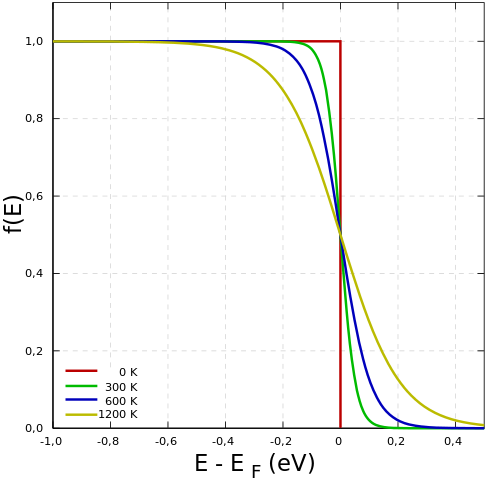
\includegraphics[width=0.5\textwidth]{fig/fermi}
        \caption{Fermi-Verteilung}
        \label{fig:fermi}
    \end{figure}

%--------------------------------------------------------------------------------
%--------------------------------------------------------------------------------
%--------------------------------------------------------------------------------
\section{Halbleiterdioden - Kapitel 5}
\subsection{PN-Übergang \todo{5x}}\label{k5:pn}
    
    \subsubsection{Raumladungszone}
	Elektronen aus dem \textit{n}-dotierten Bereich diffundieren zum \textit{p}-dotierten Bereich was zu einer Elektronenverarmung der \textit{n}-seitigen Randzone führt. 
	Dadurch wird die \textit{n} Seite positiv aufgeladen. Umgekehrt kommt es zu einer Löcherverarmung auf der \textit{p} Seite und somit zu einer negativen Aufladung dort. 
    Dadurch entsteht am Übergang eine hochohmige Verarmungszone, die sogenannte \textit{Raumladungszone} (RLZ).
    Diese Raumladung erzeugt ein Feld, welches der weiteren Diffusion von Ladungsträgern entgegenwirkt. Das Maximum der elektrischen Feldstärke liegt an der \textit{pn}-Grenze (\ref{fig:raumladungszone} b).
    
    Durch dieses elektrische Feld entsteht eine Potenzialdifferenz welche auch als \textit{Diffusionsspannung} bezeichnet wird berechnet sich folgendermaßen berechnet:
    \begin{equation}
        U_D = \varphi_2 - \varphi_1 = \int{x_1}^{x_2} E \cdot dx
    \end{equation}

           \begin{figure}[H]
        \centering
        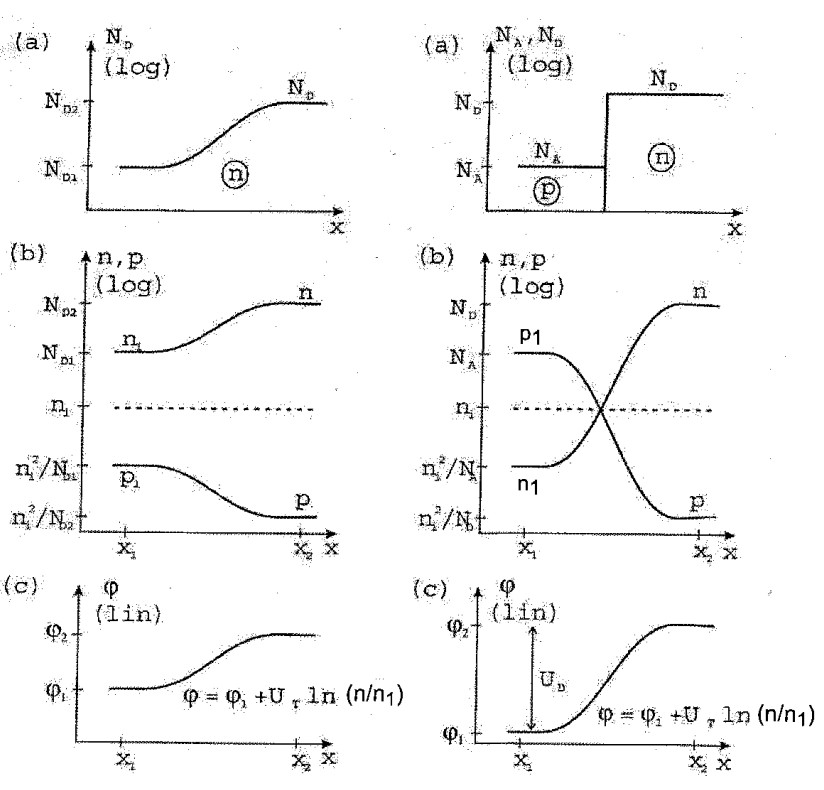
\includegraphics[width=0.5\textwidth]{fig/pnuebergang.jpg}
        \caption{linkes Bild: $nn^+$ -Übergang. Rechtes Bild: \textit{pn}-Übergang. (a) Dotierung (b) Ladungsträgerdichten (c) Potenzialverlauf}
        \label{fig:pnuebergang}
    \end{figure}
    
	$U_D$ in Silizium bei Zimmertemperatur beträgt ca. 0.8V 
    \begin{figure}[H]
        \centering
        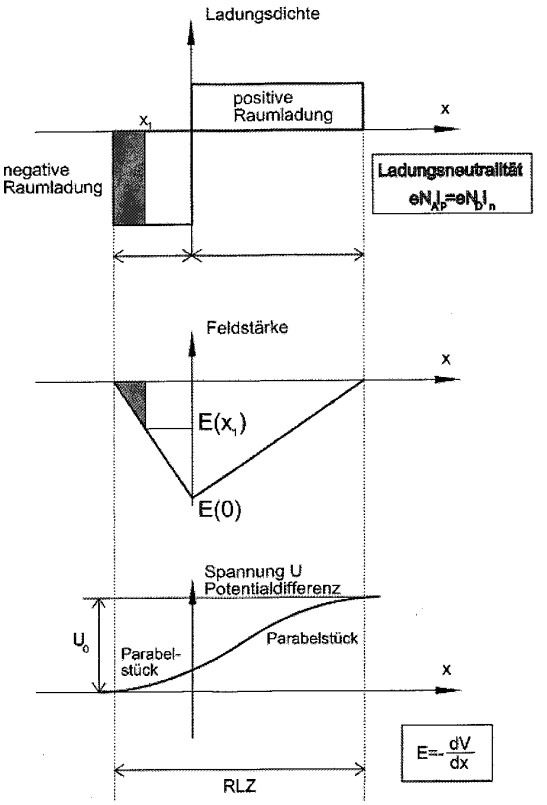
\includegraphics[width=0.5\textwidth]{fig/raumladungszone}
        \caption{Raumladungsdichte (a), Feldstärke (b) und Potenzial (c) am \textit{pn}-Übergang}
        \label{fig:raumladungszone}
    \end{figure}
    
       \begin{figure}[H]
        \centering
        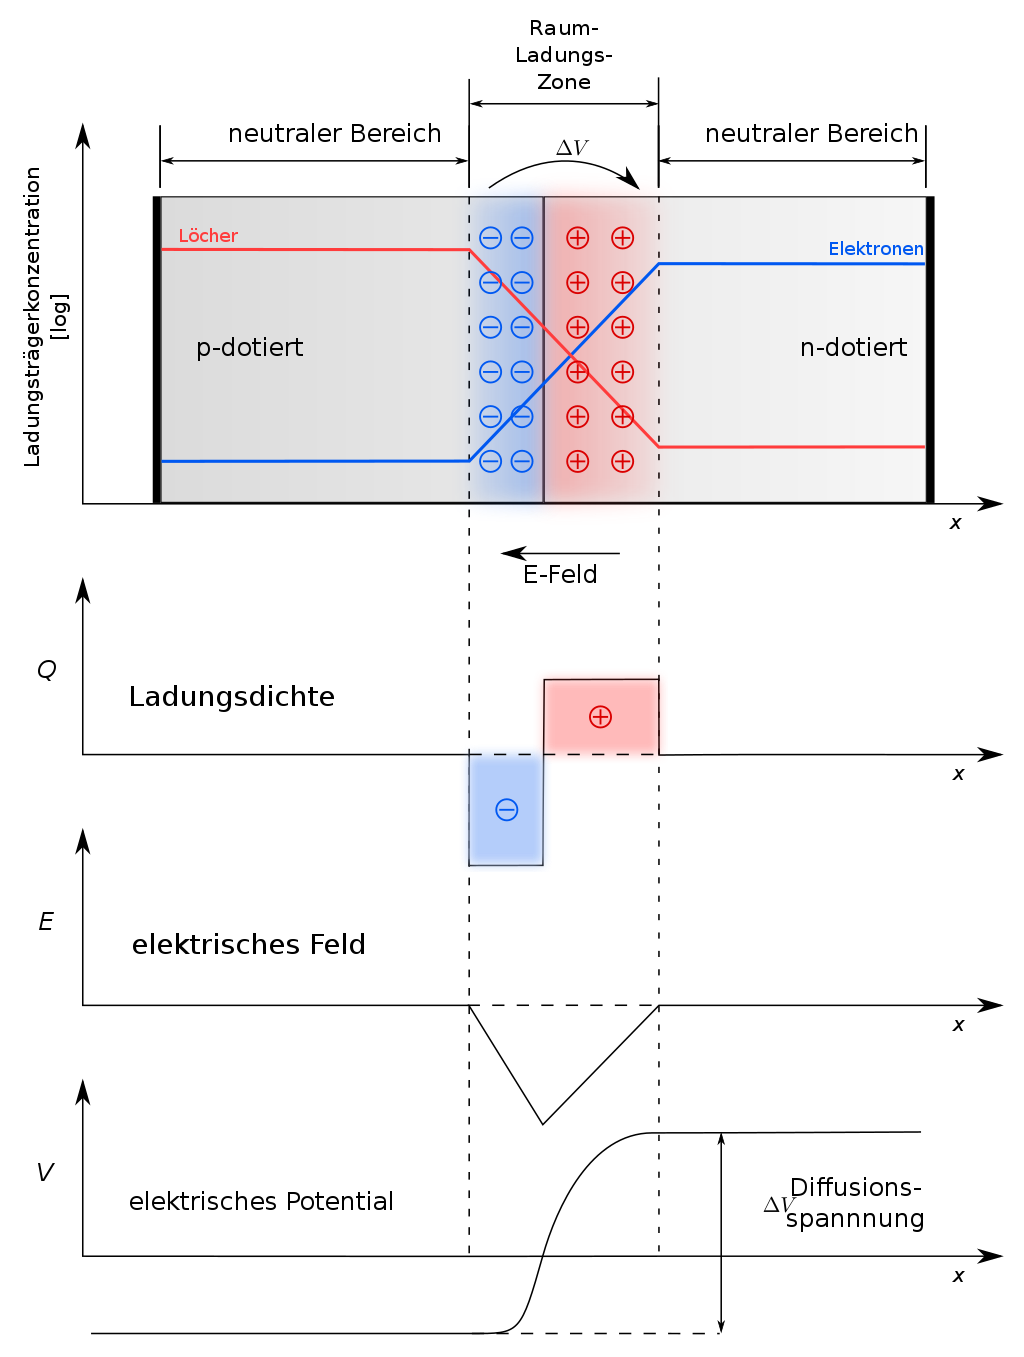
\includegraphics[width=0.5\textwidth]{fig/raumladungszone-wiki}
        \caption{Nochmal die Raumladungszone, diesmal von Wikipedia in Bunt und Farbe}
        \label{fig:raumladungszone-wiki}
    \end{figure}


	\subsubsection{Aufzeichnen ohne externe Spannung}
	Läuft wohl auf das darstellen der Raumladungszone und des elektrischen Feldes wie in \autoref{fig:raumladungszone-wiki} und \autoref{fig:raumladungszone} hinaus?
	Ohne externe Spannung kommt es wie oben beschrieben zur Ausbildung einer Raumladungszone. Bei dieser wandern die Elektronen aus dem n-Halbleiter zu den Löchern des p-Halbleiters und umgekehrt. Dabei entsteht eine Zone ohne freie Ladungsträger - eben die Raumladungszone. 
	
	\subsubsection{Diagramm dazu, wo auf x-Achse Ort (Verlauf von pn Übergang) und auf der y-Achse Dichte der freien Elektronen}
       \begin{figure}[H]
        \centering
        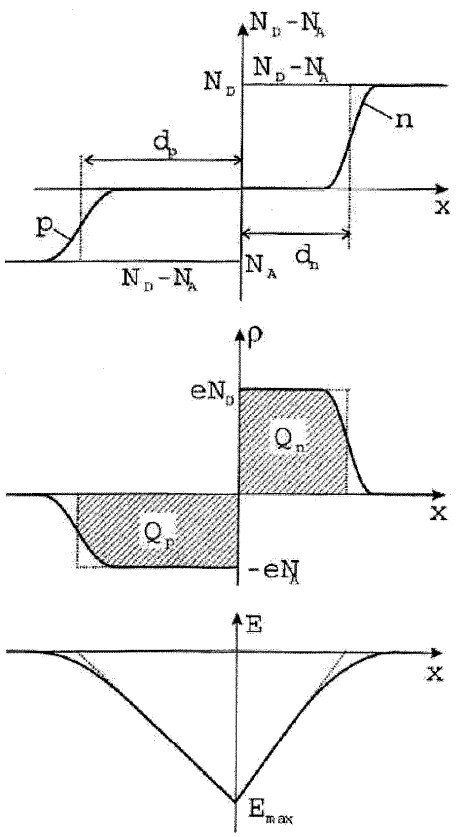
\includegraphics[width=0.5\textwidth]{fig/dotierungsVerlauf}
        \caption{Verlauf der Dotierung, der Trägerdichten \textit{n} und \textit{p}, der Raumladung $\rho$ und der Feldstärke E am abrupten \textit{pn}-Übergang. Beachten Sie, dass hier die Dichten linear aufgetragen sind.}
        \label{fig:dotierungsVerlauf}
    \end{figure}

	Hier kann man entweder mit \autoref{fig:raumladungszone-wiki} und \autoref{fig:raumladungszone} beginnen.
	Mehr Sinn macht es aber wahrscheinlich \autoref{fig:pnuebergang} aufzuzeichnen, oder sich auf \autoref{fig:dotierungsVerlauf} zu beziehen. 
	Dort kann man mit der Dotierung beginnen (diskreter Sprung, da p und n dotiert!) und die zweite Reihe stellt dann die Ladungsträgerdichte dar. Achtung, die Dichten sind logarithmisch angegeben!
	
	$N_A$ (p-Halbleiter) und $N_D$ (n-Halbleiter) stellen jeweils die Dotierungen dar, der Sprung stellt den Dotierungsverlauf / Übergang von p auf n dar.
	$n_i$ wird \textit{Intrinsic}-Zahl oder auch Eigenleitungsdichte genannt und beschreibt die Trägerdichte im undotierten Halbleiter und wird detailliert in Kapitel 3 diskutiert bzw. eingeführt. 
	
	Wikipedia hat dazu folgende Definition: Die Eigenleitungsdichte ist die charakterisierende Materialeigenschaft eines Halbleiters mit Blick auf seine elektrische Leitfähigkeit.
	Die Eigenleitungsdichte beschreibt den Mindestwert der elektrischen Leitfähigkeit, die tatsächliche Leitfähigkeit kann höher liegen (durch Verunreinigung, Dotierung). Diese Störstellenleitung (eben durch Dotierung) liegt üblicherweise um mehrere Größenordnungen über der Eigenleitung. 
	
	\subsubsection{Größenordnung einschätzen: Abstand von Elektronen, Größe von RLZ (normaler PN Übergang, Tunneldiode), Elektronendichte im HL}
	Ist eventuell in Kapitel 3 besprochen?
	
	\subsubsection{Skizze Flussrichtung, Sperrichtung, Raumladungszone}
    
       \begin{figure}[H]
        \centering
        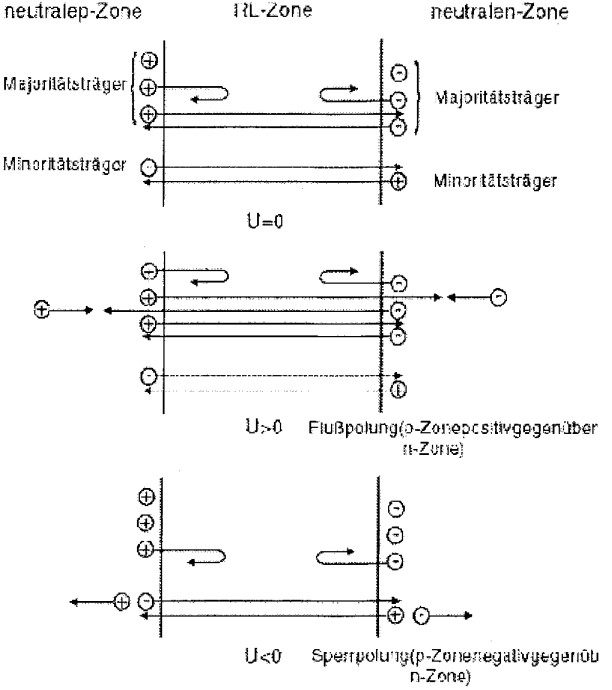
\includegraphics[width=0.5\textwidth]{fig/pn-betriebszustande}
        \caption{Betriebszustände des pn-Übergangs (oben) $U = 0$ (mitte) Flußpolung $U > 0$, p-Zone positiv gegenüber n-Zone (unten) Sperrpolung $U < 0$, p-Zone negativ gegenüber n-Zone}
        \label{fig:pn-betriebszustände}
    \end{figure}

	\subsubsection{Skalen, logarithmisch, linear, Größenordnung}
	\autoref{fig:dotierungsVerlauf} stellt die Raumladungszone linear dar, während \autoref{fig:pnuebergang} mit einer logarithmischen Darstellung arbeitet.
	Größenordungen werden wahrscheinlich wieder in Kapitel 3 erwähnt. 
	
	\subsubsection{Freie Elektronen}
	
	\subsubsection{Anzahl}
	\subsubsection{Dotierung}
	

	
\subsection{Diodenkennlinie \todo{0x}}\label{k5:diode}
Durch die Polung in Durchlassrichtung treibt die äußere Spannung sowohl die Elektronen aus dem n-Gebiet, als auch die Löcher aus dem p-Gebiet auf die Raumladungszone zu, die somit wieder bewegliche Ladungsträger enthält und ihre Sperrwirkung verliert.  
    \subsubsection{Warum exponentiell?}
    \subsubsection{Verlauf der Kapazit\"at einer Diode als Funktion der Spannung}
    \subsubsection{Wie sehen die Ladungen bei anlegen einer Spannung aus?}
    \subsubsection{Massenwirkungsgesetz}

\subsection{Banddiagramm für PN ohne Spannung \todo{1x}}\label{k5:pnBand}

\subsection{Tunneldiode \todo{4x}}\label{k5:tunnelDiode}
    \subsubsection{Banddiagramm ohne externe Spannung}
    \subsubsection{was passiert, wenn 25mV in Flussrichtung angelegt werden?}
    \subsubsection{im Banddiagramm Konstellation aufzeichnen, wo Maximum und Minimum in Kennlinie auftreten}
    
    \subsubsection{Dicke Raumladungszone Dotierung}
    \subsubsection{Wie groß ist die Bandlücke in Volt}
    \subsubsection{Kennlinie der Tunneldiode}
    \subsubsection{Kennlinie einer normalen Diode}
    
    \subsubsection{Ferminiveau (Skizze)}
    \subsubsection{Valenzband}
    \subsubsection{Leitungsband}
    \subsubsection{Ef aufzeichnen}

    \subsubsection{Warum Tunneldiode? Was tunnelt wo und wann? Was erhöht die Wahrscheinlichkeit?}

\subsection{Tunneleffekt \todo{1x}}\label{k5:tunnelEffekt}
    \subsubsection{Flussspannung}
    \subsubsection{Energieerhaltung}
    \subsubsection{Endliche Barriere}
    \subsubsection{Einfaches Tunneln}

\subsection{Schottky-Kontakt-Diode \todo{0x}}\label{k5:schottky}

\subsection{Backward-Diode \todo{0x}}\label{k5:backward}

\subsection{Heterostrukturen \todo{0x}}\label{k5:heterostrukturen}


%--------------------------------------------------------------------------------
%--------------------------------------------------------------------------------
%--------------------------------------------------------------------------------
\section{Transistoren - Kapitel 6}
\subsection{Funktion von Bipolartransistoren \todo{1x}}\label{k6:bipolar}
    \subsubsection{Funktionionsweise}
    \subsubsection{Skizze}
    \subsubsection{Warum wird er als Verst\"arker eingesetzt?}
\subsection{MOS-Struktur und Inversion \todo{2x}}\label{k6:mosInversion}

    \subsubsection{Wann spricht man von Inversion}
    \subsubsection{Leitungsband, Valenzband, Ef aufzeichnen}

\subsection{Diffusions-Dreieck beim Transistor \todo{0x}}\label{k6:diffusionsdreieck}
    \subsubsection{Warum fast linear?} exponential-Funktion im Ursprung ann\"ahernd linear
    \subsubsection{Was w\"are wenn die Basisl\"ange gr\"o{\ss}er als die Diffusionsl\"ange w\"are?} Man h\"atte die Wirkung von 2 Dioden und keinen Transistoreffekt mehr.

\subsection{Feldeffekt-Transistor \todo{0x}}\label{k6:fet}

\subsection{MOS-FET \todo{0x}}\label{k6:mosfet}
    \subsubsection{Aufbau}
    \subsubsection{Bandstruktur}

\subsection{MES-FET \todo{0x}}\label{k6:mesfet}

\subsection{Early-Effekt \todo{0x}}\label{k6:early}

\subsection{JFET \todo{0x}}\label{k6:jfet}

%--------------------------------------------------------------------------------
%--------------------------------------------------------------------------------
%--------------------------------------------------------------------------------
\section{Ohne Kapitel}
\end{document}
